\documentclass[compress,10pt]{beamer}

%-----------------------------------------------------------------------------
% Packages
%-----------------------------------------------------------------------------

\usepackage[english]{babel}
\usepackage[latin1]{inputenc}
\usepackage{color}
\usepackage{times}
\usepackage{array}
\usepackage[T1]{fontenc}
% \usepackage{fancyvrb}                      % Fancy verbatim for inputting source code
\usepackage{amsmath}
\usepackage{amssymb}
\usepackage{ifpdf}                         % different options for pdflatex
\usepackage{graphicx}
\usepackage{pgf}
\usepackage{multirow}
\usepackage{colortbl}

%\usepackage{psfrag}
\usepackage{subfigure} 
%\usepackage{epsfig} 
%-----------------------------------------------------------------------------
% Definitions
%-----------------------------------------------------------------------------

\newcommand{\dd}[2]{{\frac{\partial #1}{\partial #2}}}
\newcommand{\ddn}[2]{{\frac{d #1}{d #2}}}
\newcommand{\dddn}[2]{{\frac{d^2 #1}{d #2 ^2}}}
\newcommand{\omg}{\scriptscriptstyle\Omega}

\definecolor{mygreen}{rgb}{0.0,0.7,0.0}
\definecolor{dgreen}{rgb}{0.0,0.4,0.0}
\definecolor{myred}{rgb}{0.8,0.0,0.0}
\definecolor{nblue}{rgb}{0.0,0.0,0.55}
\definecolor{col1}{rgb}{0.1,0.9,0.}
\definecolor{col2}{rgb}{0.1,0.7,0.2}
\definecolor{col3}{rgb}{0.8,0.0,0.2}
\definecolor{col4}{rgb}{0.1,0.5,0.4}

\newcommand{\greentriag}{ \textcolor{green}{$\blacktriangleright$}\hspace{2pt}}
\newcommand{\redtriag}{ \textcolor{myred}{$\blacktriangleright$}\hspace{2pt}}

% counter for broken enumerates
\newcounter{saveenumi}

%-----------------------------------------------------------------------------
% Search paths for figures
%-----------------------------------------------------------------------------
\DeclareGraphicsExtensions{.png,.pdf,.jpg}

%-----------------------------------------------------------------------------
% Beamer style settings
%-----------------------------------------------------------------------------
\mode<presentation>
{
  \usetheme{vkialt}
}

% turnof navigation symbols
\setbeamertemplate{navigation symbols}{}

% title each section
 \AtBeginSection{
    \begin{frame}
    \tableofcontents[sectionstyle=show/shaded%
                    ,subsectionstyle=show/show/shaded]
    \end{frame}
} 
%-----------------------------------------------------------------------------
% Mathematical symbols
%-----------------------------------------------------------------------------
\newcommand{\pdif}[2]{\frac{\partial #1}{\partial #2}}
\newcommand{\bolditu}{\boldsymbol{\mathit{u}}}
\newcommand{\bolditxi}{\boldsymbol{\xi}}
\newcommand{\boldlambda}{\boldsymbol{\lambda}}
\newcommand{\bolditF}{\boldsymbol{\mathcal{F}}}
\newcommand{\boldF}{\boldsymbol{\mathit{F}}}
\newcommand{\bolditf}{\boldsymbol{\mathit{f}}}
\newcommand{\bolditS}{\boldsymbol{\mathcal{S}}}
\newcommand{\bolditD}{\boldsymbol{\mathcal{D}}}
\newcommand{\bolditk}{\boldsymbol{\mathit{k}}}
\newcommand{\bolditx}{\boldsymbol{\mathit{x}}}
\newcommand{\bolditn}{\boldsymbol{\mathit{n}}}
\newcommand{\bolditv}{\boldsymbol{\mathit{v}}}
\newcommand{\RDS}{\mathcal{RDS}}
% \newcommand{\boldw}{\boldsymbol{\mathit{w}}}

% this put thick lines around tables
\newdimen\tlusta
\setlength{\tlusta}{1pt}
\makeatletter
\def\Hline{\noalign{\ifnum0=`}\fi\hrule \@height \tlusta
\futurelet \@tempa\@xhline}
\makeatother

%-----------------------------------------------------------------------------
% Title, Authors and such
%-----------------------------------------------------------------------------
\title[ICP-COOLFluiD tutorial]{How to simulate a Plasmatron test with COOLFluiD}%
\author[N. Villedieu]{N. Villedieu and A. Lani}
 \institute[von Karman Institute]{
\begin{center}
\begin{minipage}{0.2\textheight}
 
\includegraphics[height=1.5cm]{vkilogo}
\end{minipage}
\end{center}
}

%----------------------------------------------------------------------------
\begin{document}
 
%----------------------------------------------------------------------------
\frame{\titlepage}
%----------------------------------------------------------------------------
\frame
{
\frametitle{Outline}
\tableofcontents
}

\section{Starting with COOLFluiD}
\begin{frame}[fragile]
\frametitle{How to install COOLFluiD?}
\begin{block}{Loading of the sources and compilation}
\begin{itemize}
\item The first step is \textcolor{blue}{ALWAYS}: \textcolor{blue}{\texttt{\small{module load cf2-2012.3/lammpi}}}
\item To get the \textcolor{blue}{sources}:
\begin{itemize}
 \item For the kernel (part of the code that is common to every applications)
\begin{verbatim}
 svn co 
    https://coolfluidsrv.vki.ac.be/svn/
        coolfluid/Sources/Kernel/trunk COOLFLUID
\end{verbatim}
\item For the \textcolor{blue}{plugins}:
\begin{enumerate}
 \item \textcolor{blue}{Adapt the coolfluid.conf} and put it in the COOLFLUID directory
 \item \texttt{cd COOLFLUID}
 \item \texttt{./prepare.pl --mods-up}
\end{enumerate}
\item \textcolor{blue}{Compilation}:
\begin{enumerate}
 \item \texttt{./prepare.pl --build=release}
 \item \texttt{cd builds/x86$\_$64/release/}
 \item \texttt{make -j6}
\end{enumerate}
\end{itemize}
\end{itemize}
\end{block}
\end{frame}

\begin{frame}[fragile]
\frametitle{How to install COOLFluiD}
\begin{block}{Adaptation of coolfluid.conf}
 \begin{itemize}
  \item Path of the two first lines:
\texttt{coolfluid$\_$dir=/villedie/workspace/COOLFLUID}
\texttt{basebuild$\_$dir=/villedie/workspace/COOLFLUID/
\hspace*{6cm}builds/x86$\_$64}
  \item The path to the dependencies
\texttt{mpi$\_$dir=/ardisksrv1/projects/cf2/2012.3/lam}
 \end{itemize}

\end{block}
\begin{block}{The special case of Rocks5}
 \begin{itemize}
  \item \textcolor{blue}{Read the wiki} about rocks5
  \item Get a node \textcolor{blue}{\texttt{qcompile}}
  \item Follow the steps mentioned in slide 1 
 \end{itemize}
\end{block}

\end{frame}

\begin{frame}[fragile]
\frametitle{How to run COOLFluiD}
\begin{block}{}
 \begin{itemize}
  \item \textcolor{blue}{\texttt{module load coolfluid2/2010.0}}
  \item If needed \texttt{lamboot}
  \item \textcolor{blue}{Create symbolic links to the executable}
\begin{verbatim}
      ln -sf /villedie/workspace/COOLFLUID/
            builds/x86_64/release/src/
            Solver/coolfluid-solver .
      ln -sf /villedie/workspace/COOLFLUID/
            builds/x86_64/release/src/
            Solver/coolfluid-solver.xml .
\end{verbatim}
    \item \textcolor{blue}{Run} 
      \begin{itemize}
	\item In serial: 
\begin{verbatim}
./coolfluid-solver --scase ./torch_4_res.CFcase
\end{verbatim}
	\item In parallel (it may be necessary to do lamboot first) : 
\begin{verbatim}
mpirun -np 2 ./coolfluid-solver --scase 
                          ./torch_4_res.CFcase
\end{verbatim}
      \end{itemize}
 \end{itemize}
\end{block}
\end{frame}

\section{Simulation of the Plasmatron facility}
\begin{frame}[fragile]
 \frametitle{How to simulate a Plasmatron test}
\begin{block}{What can we simulate?}
\begin{itemize}
\item It is possible to simulate the \textcolor{blue}{torch+chamber+probe}
\item The flow is considered as \textcolor{blue}{LTE}
\end{itemize}
\end{block}
\begin{block}{Steps}
\begin{enumerate}
 \item Doing the mesh
 \item Simulation of the torch with simple Euler boundary conditions
 \item Torch with full boundary conditions
 \item Extrapolation of the torch solution in the chamber
 \item Chamber with $1^{st}$ order scheme
 \item Chamber with $2^{nd}$ order scheme
\end{enumerate}
\end{block}
\end{frame}

 \subsection{Mesh requirements}
 \begin{frame}
  \frametitle{How to do the mesh}
 \begin{block}{Few instructions for Gambit}
 \begin{itemize}
  \item It is advisable to do the \textcolor{blue}{mesh on a scaled} ($\approx 100$) \textcolor{blue}{geometry} 
  \item You should register all the boundaries:
 \begin{itemize} 
 \item Click Solver $\rightarrow$ generic
 \item Click the green button on the left (in Operation) $\rightarrow$ white button in zones 
 \item Register all your boundaries name
 \end{itemize}
 \item Save the mesh in .neu:
       Click File $\rightarrow$ export $\rightarrow$ mesh  and give a name
 \end{itemize}
 \end{block}
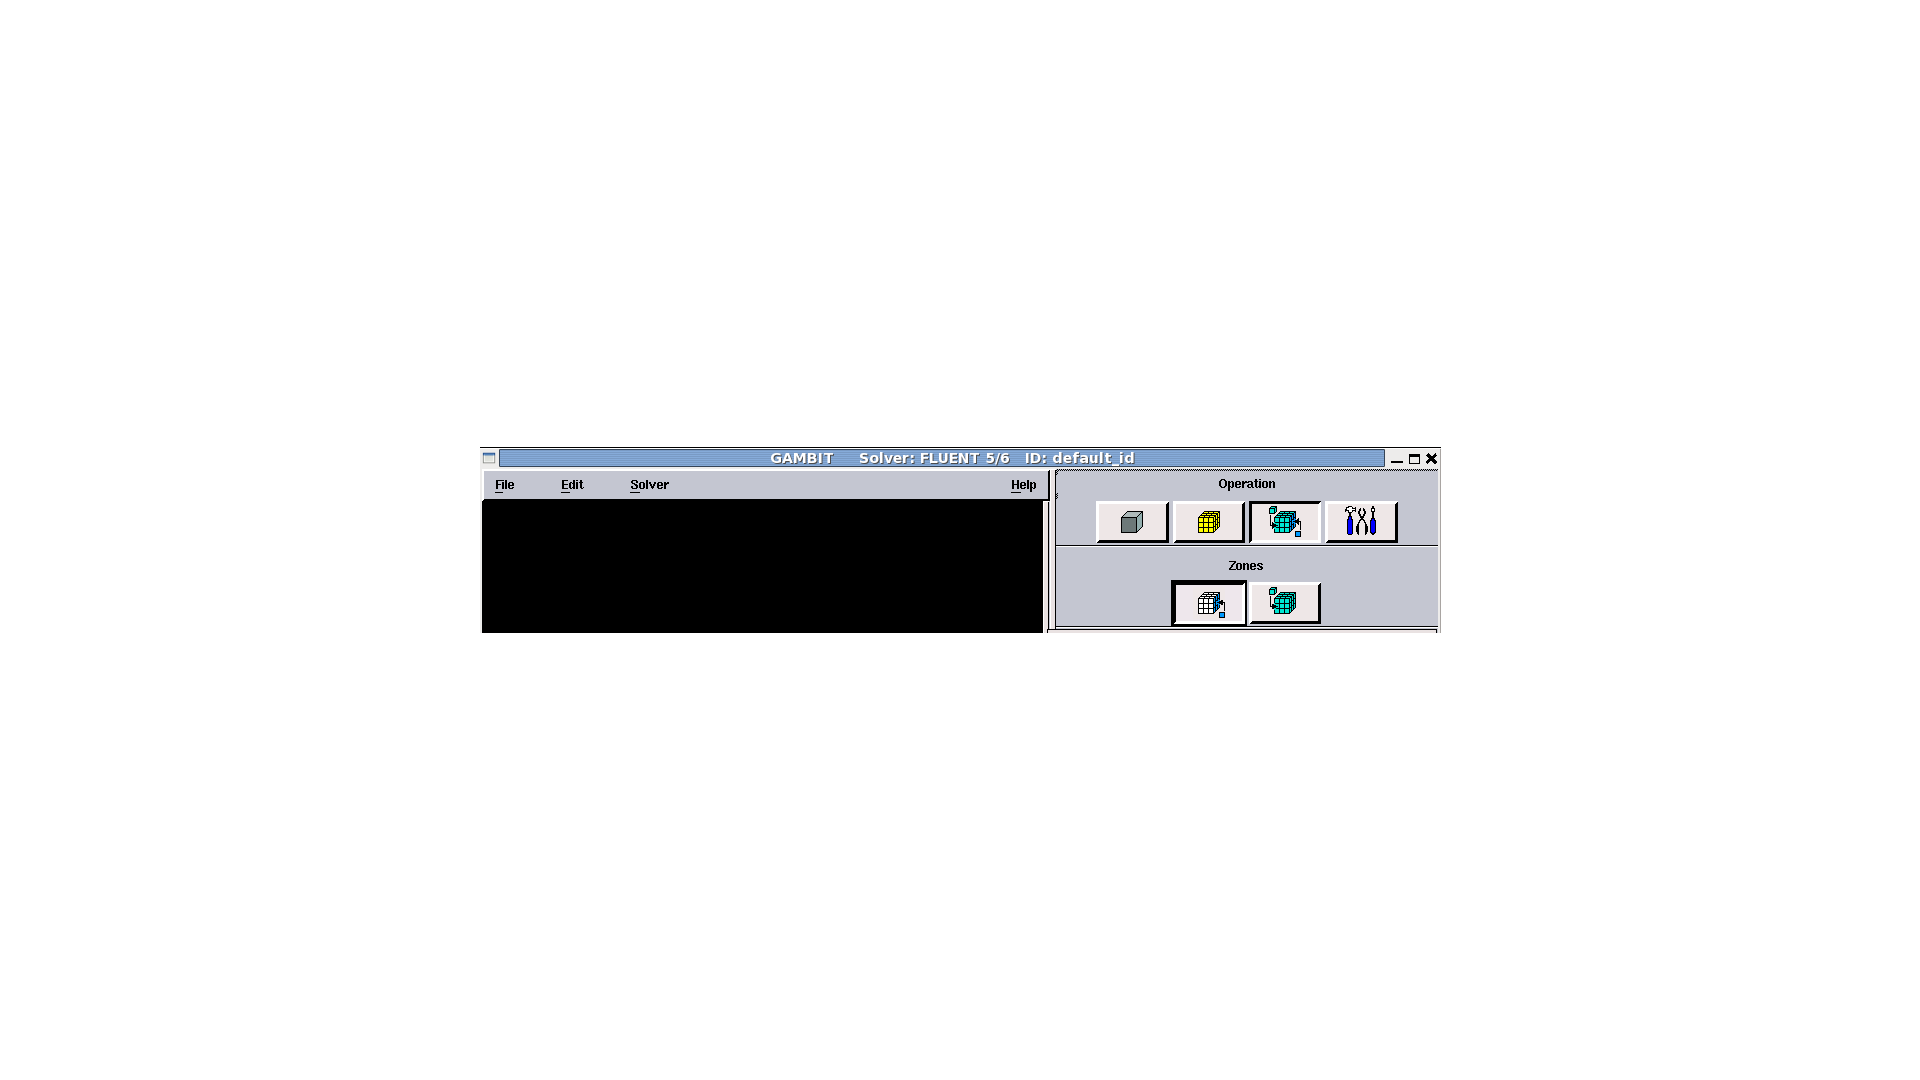
\includegraphics[width=1.2\textwidth,viewport= 200 250 1200 500,clip]{gambit1.png}
 \end{frame}

\begin{frame}[fragile]
 \frametitle{How to do the mesh}
\begin{block}{ You need to do two meshes}
\begin{itemize}
\item One for the torch
\item One for the torch+chamber+probe: The \textcolor{blue}{torch block} should keep \textcolor{blue}{the same}
\end{itemize}
\end{block}
\begin{block}{Mesh requirements for the torch}
\begin{itemize}
 \item The mesh should not be very fine: $1800<\sharp \textrm{nodes}<2500$
 \item It should be refined near the walls and the outlet
\end{itemize}
\end{block}
\begin{center}
\vspace*{-0.1cm}
  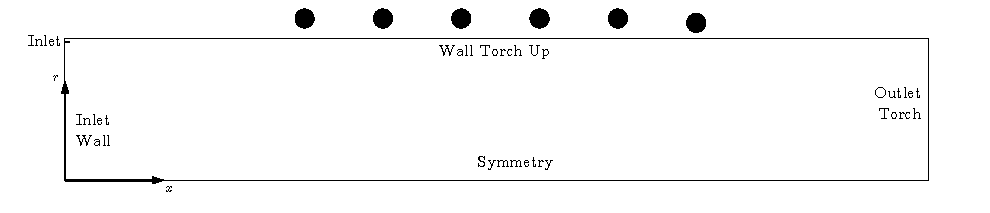
\includegraphics[width=\textwidth]{geom_torch.pdf}\\
\vspace*{-0.1cm}
  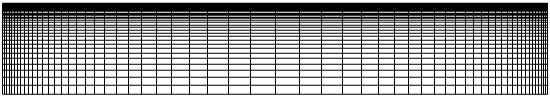
\includegraphics[width=0.8\textwidth]{mesh_torch_3.png}
\end{center}
\end{frame}
 
 \begin{frame}
 \frametitle{Meshing Torch+chamber+probe}
 \begin{block}{Definition of the domain}
  \begin{itemize}
   \item Only the part of the chamber close to the probe is modeled
    \begin{itemize}
    \item Probe at $x=445mm$ $\Rightarrow$ domain is cut at $x=1210mm$
    \item Ray of the probe $25mm$ $\Rightarrow$ the chamber is cut at $y=160mm$ 
  \end{itemize}
\end{itemize}
 \end{block}
%\vspace*{-0.2cm}
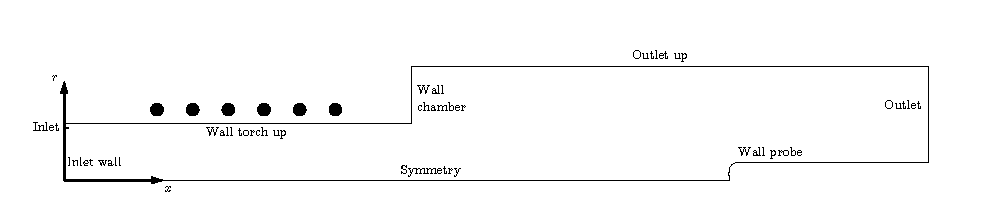
\includegraphics[width=\textwidth,viewport= 10 10 450 80,clip]{geometry_compl.pdf}\\
 \begin{block}{Doing the mesh}
  \begin{itemize}
   \item Should start from the torch mesh
   \item Refine near the probe (mesh size around $5 \mu m$)
   \item Coarsening around the top boundary
  \end{itemize}
 \end{block}
%\vspace*{-0.2cm}
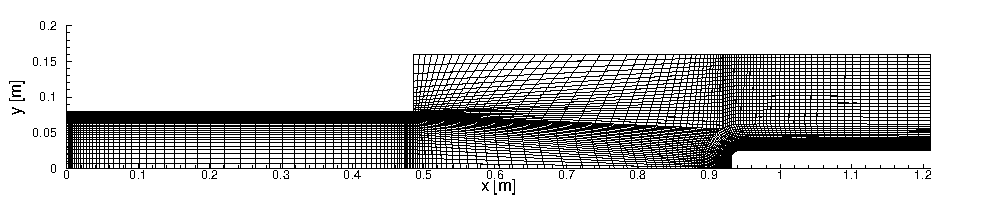
\includegraphics[width=0.8\textwidth,viewport= 0 10 450 80,clip]{chamber_pb_mesh.pdf}
 \end{frame}

\subsection{Simulation of the torch}
\begin{frame}
\frametitle{First phase of the simulation}
  \begin{block}{\texttt{torch$\_$4$.$CFcase}}
 The CFcase is divided in two parts:
   \begin{itemize}
    \item First part, does not need to be changed (setup of FV, LTE...)
    \item \textcolor{blue}{Second part, needs to be adapted to your case}
   \end{itemize}
 \end{block}
 \begin{block}{Loading the mesh}
\texttt{\small{Simulator.SubSystem.Default.listTRS = InnerFaces...}}
\texttt{\small{Simulator.SubSystem.CFmeshFileReader.Data.FileName = 
                      \hspace*{8cm}      torch$\_$4.CFmesh}}\\
\begin{itemize}
 \item The extension should be {\bf{.CFmesh}}
 \item If the Gambit file was done with a scaling:
\end{itemize}
\texttt{\small{Simulator.SubSystem.CFmeshFileReader.Data.
\hspace*{6cm}  ScalingFactor=1000}}
 \end{block}
 \end{frame}

\begin{frame}
\frametitle{First phase of the simulation}
  \begin{block}{Stopping the simulation}
  It is possible to setup a condition on the residual:
  \texttt{\small{Simulator.SubSystem.StopCondition=Norm}}
\texttt{\small{Simulator.SubSystem.Norm.valueNorm=-2.0}}
\begin{itemize}
 \item Here it should be \textcolor{blue}{stopped} it \textcolor{blue}{by hand} (Clt + C) when
temperature and streamlines are as follows (around 500-1500 iterations).  
\end{itemize}
\vspace*{-0.2cm}
 \end{block}
 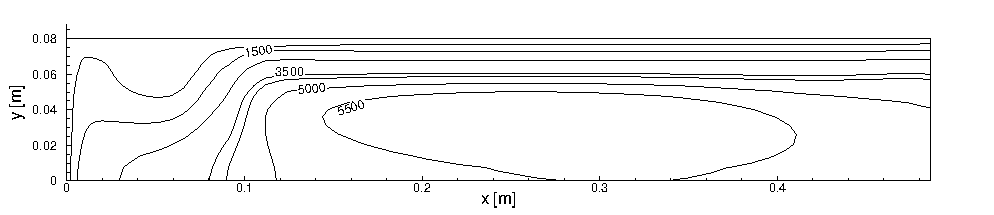
\includegraphics[width=\textwidth]{torch_T_nc.pdf}\\
\vspace*{-0.2cm}
 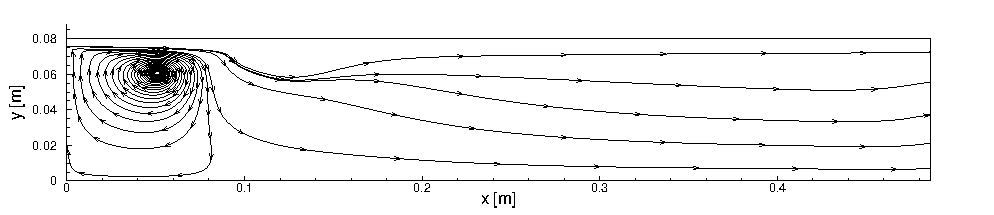
\includegraphics[width=\textwidth]{torch_SL_nc.pdf}
 \end{frame}

\begin{frame}
\frametitle{First phase of the simulation}
\vspace*{-0.1cm}
  \begin{block}{CFL}
   For this phase the best is to use an interactive CFL
\texttt{\small{Simulator.SubSystem.NewtonIterator.Data.CFL.
\hspace*{6cm} ComputeCFL=Interactive}}
\texttt{\small{Simulator.SubSystem.NewtonIterator.Data.CFL.
\hspace*{6cm} Interactive.CFL=0.0001}}
\texttt{\small{Simulator.SubSystem.InteractiveParamReader.
\hspace*{6cm} FileName=./torch.inter}}
\texttt{\small{Simulator.SubSystem.InteractiveParamReader.readRate=5}}\\
The \textcolor{blue}{CFL should change slowly}
  \end{block}
\vspace*{-0.1cm}
  \begin{block}{Outputs}
It is possible to use several outputs: COOFluiD, tecplot, paraview....
\texttt{\small{Simulator.SubSystem.OutputFormat=Tecplot$\,$CFmesh}}\\
You can define file names....\\
\texttt{\small{Simulator.SubSystem.CFmesh.FileName=torch$\_$4-out.CFmesh}}\\
\texttt{\small{Simulator.SubSystem.Tecplot.SaveRate=50}}\\
\texttt{\small{Simulator.SubSystem.Tecplot.Data.SurfaceTRS=Wall$\_$torch$\_$in}}\\
  \end{block}
 \end{frame}
\begin{frame}
\frametitle{First phase of the simulation}
\begin{block}{Initialization}
 \texttt{\small{Simulator.SubSystem.CellCenterFVM.InitComds=InitState}}
 \texttt{\small{Simulator.SubSystem.CellCenterFVM.InitNames=InField}}
 \texttt{\small{Simulator.SubSystem.CellCenterFVM.InField.applyTRS
\hspace*{6cm}=InnerFaces}}
 \texttt{\small{Simulator.SubSystem.CellCenterFVM.InField.Vars=x$\,$y}}
 \texttt{\small{Simulator.SubSystem.CellCenterFVM.InField.Def=0. $\backslash$ \\
                                               \hspace*{2cm} if(y>.075,if(y<.08,100.,0.),if(x>.2,0.,0.))$\backslash$ \\
                                               \hspace*{5cm} 0.$\backslash$ \\
						\hspace*{5cm} ...}}
\end{block}
 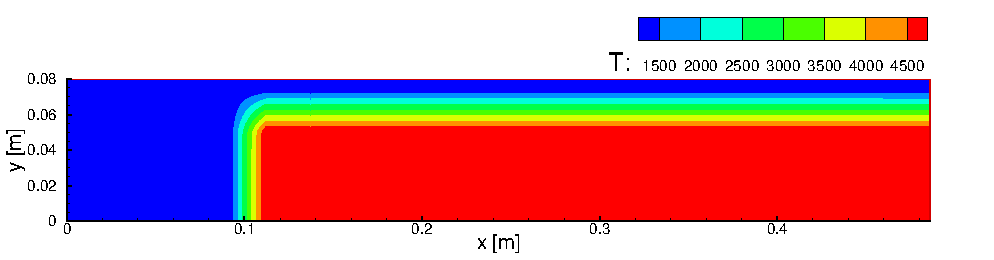
\includegraphics[width=\textwidth]{torch_T_initial.pdf}
\end{frame}
\begin{frame}
\frametitle{First phase of the simulation}
\vspace*{-0.2cm}
  \begin{block}{Extrapolation}
\begin{itemize}
\item Extrapolation from cell centers to nodes for the viscous gradients and visualization \\
\hspace*{-0.2cm}\texttt{\small{Simulator.SubSystem.CellCenterFVM.Data.
\hspace*{0.1cm} NodalExtrapolation=DistanceBasedGMoveMultiTRS}}\\
\hspace*{-0.2cm}\texttt{\small{Simulator.SubSystem.CellCenterFVM.Data.
\hspace*{0.1cm} DistanceBasedGMoveMultiTRS.TrsPriorityList=Wall$\_$torch...}}\\
\hspace*{-0.2cm}\texttt{\small{Simulator.SubSystem.CellCenterFVM.Data.
\hspace*{0.1cm} DistanceBasedGMoveMultiTRS.TRSName=Wall$\_$torch...}}
 \item Impose strongly \textcolor{blue}{wall temperature}
 \item Impose strongly \textcolor{blue}{electro-magnetic field to zero} (only in this transient phase)\\
\texttt{\small{Simulator.SubSystem.CellCenterFVM.Data.
\hspace*{0.1cm} DistanceBasedGMoveMultiTRS.Wall$\_$torch$\_$in.
\hspace*{6cm} ValuesIdx=1$\,$2$\,$3$\,$4$\,$5}}
\texttt{\small{Simulator.SubSystem.CellCenterFVM.Data.
\hspace*{0.5cm} DistanceBasedGMoveMultiTRS.Wall$\_$torch$\_$up.
\hspace*{6cm} Values=0$\,$0$\,$350$\,$0$\,$0}}
\end{itemize}
  \end{block}
 \end{frame}

\begin{frame}
\frametitle{First phase of the simulation}
\begin{block}{Boundary conditions}
\begin{itemize}
 \item List of the commands:\\
\hspace*{-0.5cm} \texttt{\small{Simulator.SubSystem.CellCenterFVM.BcComds=MirrorICPFVMCC}}
 \item List of names:\\
\hspace*{-0.5cm}  \texttt{\small{Simulator.SubSystem.CellCenterFVM.BcNames=BcTorchWallUp}}
 \item TRS where it is applied:
\hspace*{-0.5cm}  \texttt{\small{Simulator.SubSystem.CellCenterFVM.BcOutletTorch
  \hspace*{6cm}.applyTRS=Outlet$\_$torch}}
\end{itemize}
\end{block}
 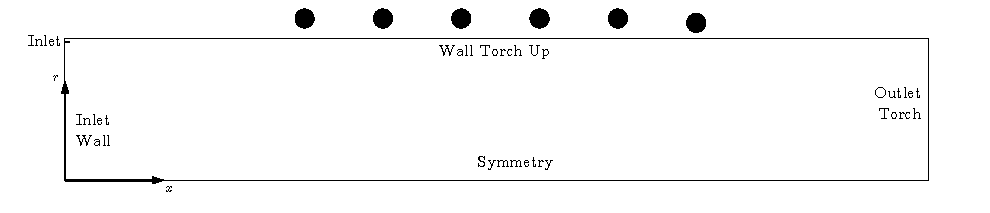
\includegraphics[width=\textwidth]{geom_torch.pdf}
\end{frame}




\begin{frame}
\frametitle{First phase of the simulation}
\begin{block}{Outlet Torch:\texttt{SubOutletICP2DPuvtFVMCC}}
\begin{itemize}
\item At the Outlet we impose no pressure perturbations:\\
  \texttt{\small{Simulator.SubSystem.CellCenterFVM.BcOutletTorch.P=0.0}}
\end{itemize}
\end{block}
\begin{block}{Walls:\texttt{NoSlipWallIsothermalICPPvtFVMCC}}
\begin{itemize}
\item At the wall we impose isothermal temperature:\\
  \texttt{\small{Simulator.SubSystem.CellCenterFVM.BcTorchWallUp.
\hspace*{6cm}TWall=350.}}
\end{itemize}
\end{block}
 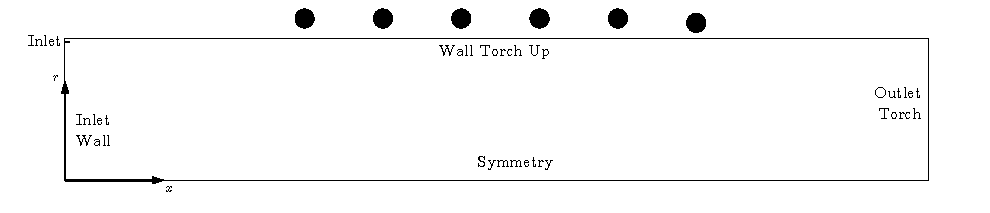
\includegraphics[width=\textwidth]{geom_torch.pdf}
\end{frame}

\begin{frame}
\frametitle{First phase of the simulation}
\begin{block}{Inlet:\texttt{SubInletICP2DPuvtUVTFVMCC}}
\begin{itemize}
\item At the inlet we imposse the mass flow, temperature and the geometry is defined\\
\texttt{\small{Simulator.SubSystem.CellCenterFVM.BcInlet.MassFlow=16.}}\\
\texttt{\small{Simulator.SubSystem.CellCenterFVM.BcInletT=350.}}\\
\texttt{\small{Simulator.SubSystem.CellCenterFVM.BcInlet.
\hspace*{6cm}InletRadii=.075$\,$.08}}\\
\end{itemize}
\end{block}
\begin{block}{Symmetry line:\texttt{MirrorICPFVMCC}}
 All radial gradients are set to zero
\end{block}

 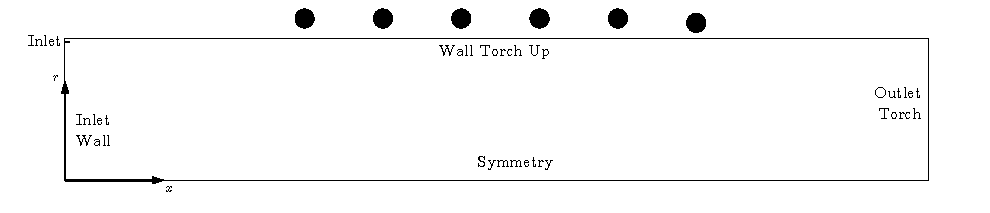
\includegraphics[width=\textwidth]{geom_torch.pdf}
\end{frame}

\begin{frame}
\frametitle{First phase of the simulation}
\begin{block}{Definition of the coils and current}
\begin{itemize}
\item Definition of the PLASMA POWER\\
\texttt{\small{Simulator.SubSystem.DataProcessing.JouleHeatSource.
\hspace*{2cm}DesiredPower=90.}}\\
\item Definition of the setup of the coils\\
\texttt{\small{Simulator.SubSystem.DataProcessing.JouleHeatSource.
\hspace*{2cm}NbCoils=6}}
\texttt{\small{Simulator.SubSystem.DataProcessing.JouleHeatSource.
\hspace*{2cm}RadiusCoils=$\,$.109$\,$.109$\,$.109$\,$.109$\,$.109$\,$.109}}
\texttt{\small{Simulator.SubSystem.DataProcessing.JouleHeatSource.
\hspace*{2cm}ZPositionCoils=.127$\,$.177$\,$.227$\,$.277$\,$.327$\,$.377}}
\item Writing the Joule Heat in a file:\\
\texttt{\small{Simulator.SubSystem.DataProcessing.JouleHeatSource.
\hspace*{2cm}OutputFileElCurrent=.$\diagdown$elCurrent.plt}}
\end{itemize}
\end{block}
\end{frame}

\begin{frame}
\frametitle{Second phase}
\begin{block}{Differences with the first phase}
 In this phase the \textcolor{blue}{electromagnetic field} is imposed to \textcolor{blue}{zero in the far-field}
by the boundary conditions.
\end{block}

\begin{block}{Setup}
\begin{itemize}
\item We use the output of the previous simulation to restart the simulation:\\
\texttt{\small{Simulator.SubSystem.CellCenterFVM.Restart=true}}
\item The Boundary conditions also modify the EM:\\
\texttt{\small{Simulator.SubSystem.CellCenterFVM.BcComds
\hspace*{2cm}=EpComputingNoSlipWallIsothermalICPPvtFVMCC}}
\end{itemize}
\end{block}
\end{frame}

\begin{frame}
 \frametitle{Second phase}
 \begin{block}{CFL}
 The CFL can be increased faster:
 \texttt{\small{Simulator.SubSystem.NewtonIterator.Data.CFL.Value=0.01}}\\
 \texttt{\small{Simulator.SubSystem.NewtonIterator.Data.CFL.
 \hspace*{2cm}ComputeCFL=Function}}\\
 \texttt{\small{Simulator.SubSystem.NewtonIterator.Data.CFL.
 \hspace*{2cm}Function.Def=if(i>80,5,1)}}\\
\begin{center} 
\begin{tabular}{lc}
 \textbf{Iteration} & \textbf{CFL} \\ \hline
 $1 \sim 10 $ & 0.01 \\ \hline
 $10 \sim 45 $ & 0.1 \\ \hline
 $45 \sim 100 $ & 1 \\ \hline
 $100 \sim 295 $ & 10 \\ \hline
 $>295$ & 100 \\ 
 \hline
 \end{tabular}
\end{center}
 \end{block}
\end{frame}
\subsection{Extrapolation of the solution to the chamber}
\begin{frame}

\frametitle{Extrapolation}
\begin{itemize}
 \item The solution in the torch is used to approximate 
the solution in the chamber
\end{itemize}
\begin{block}{Installing the code}
\begin{itemize}
 \item You need to change the path in:
\begin{itemize}
 \item build/Makefile
 \item build/CMakeFiles/initialcond.dir/depend.intern
 \item build/CMakeFiles/initialcond.dir/DependInfo.cmake
 \item build/CMakeFiles/initialcond.dir/build.make
\end{itemize}
\item Adapt mesh names in main.cpp
\item compile
\item Run: \texttt{build/initialcond}
\end{itemize}
\end{block}
  \end{frame}
\subsection{Simulation of the full geometry}

\begin{frame}
\frametitle{First Order Chamber}
\begin{itemize}
 \item The CFcase for the full geometry is very similar to the one of phase two,
the main changes are:
\begin{itemize}
 \item The TRS names and mesh name
 \item The boundary conditions:
\begin{itemize}
 \item Wall Chamber $\Rightarrow$ Isothermal wall (with an eventual blowing)
 \item Outlet up $\Rightarrow$ SubOutlet
 \item Outlet $\Rightarrow$ SuperOutlet
 \item Wall Probe $\Rightarrow$ Isothermal Wall
\end{itemize}
\end{itemize}
\end{itemize}
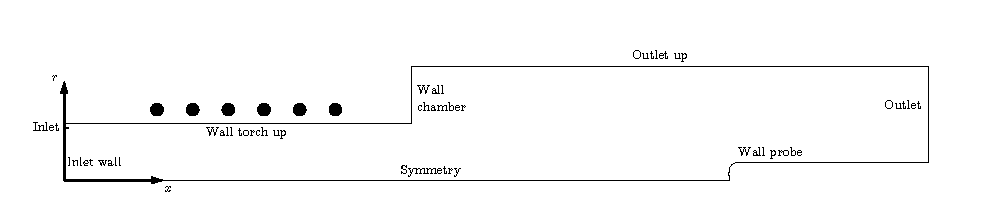
\includegraphics[width=\textwidth,viewport= 10 10 450 80,clip]{geometry_compl.pdf}
  \end{frame}

\begin{frame}
\frametitle{Second Order Chamber}
\begin{itemize}
 \item The second order simulation should start from the $1^{st}$ order one
 \end{itemize}
\begin{block}{What changes}
\begin{itemize}
 \item The polynomial reconstruction:
\texttt{\small{Simulator.SubSystem.CellCenterFVM.Data.
\hspace*{5cm}PolyRec=LinearLS2D}}
\texttt{\small{Simulator.SubSystem.CellCenterFVM.Data.
\hspace*{5cm}LinearLS2D.gradientFactor=1.}}
\item Add a limiter (because of the high gradients in temperature)
\texttt{\small{Simulator.SubSystem.CellCenterFVM.Data.LinearLS2D.
\hspace*{5cm}limitRes=-15.}}
\texttt{\small{Simulator.SubSystem.CellCenterFVM.Data.
\hspace*{5cm}Limiter=Venktn2D}}
\texttt{\small{Simulator.SubSystem.CellCenterFVM.Data.Venktn2D.
\hspace*{5cm}coeffEps=1.0}}
\item Add a condition on gradients at the boundaries
\texttt{\small{Simulator.SubSystem.CellCenterFVM.BcTorchWallIn.
\hspace*{5cm}ZeroGradientFlags=1$\,$0$\,$0$\,$0$\,$1$\,$1}}
\end{itemize}
\end{block}
\end{frame}

\begin{frame}
 \frametitle{Remarks}
\begin{block}{Is it necessary to redo this always?}
\begin{itemize}
 \item For a new geometry: YES
 \item For a geometry where solutions exists:
  \begin{itemize}
    \item For change of pressure around $2000\sim4000Pa$: NO\\
    You just need to adjust the pressure and velocity\\
\texttt{Simulator.SubSystem.ICPLTE2D.refValues = 1. 100. 100. 10000. 0.01 0.01}
\texttt{Simulator.SubSystem.ICPLTE2D.ConvTerm.uInf = 100.}
\texttt{Simulator.SubSystem.ICPLTE2D.ConvTerm.p0Inf = 10000.}
     \item For change of the power $30\sim40 kW$: NO
     \item Otherwise YES
\end{itemize}
\end{itemize}

 
\end{block}

\end{frame}

\begin{frame}
 \frametitle{Remarks}
\begin{block}{Possible issues}
It is possible that few problems occurs:
\begin{itemize}
 \item Problems around walls:
\begin{itemize}
 \item Near the probe: need for refinements
 \item Near Inlet wall: use adiabatic wall
\end{itemize}
\item Creation of a recirculation on the top region:\\
impose a small horizontal velocity out of the jet
\end{itemize}
\end{block}
\end{frame}

\section{Conclusion}
\begin{frame}
 \frametitle{Conclusion}
\begin{itemize}
 \item If you want to understand better I advise you to read:
\begin{itemize}
\item The report of Sartori: VKI SR 2010-01.
\item The report of PerisNavarro: SR 2011-22.
\end{itemize}
\item From the ICP computation, people usually want to compute the NDP's
For this I porpose to do another lecture
\end{itemize}
\end{frame}

\end{document}
